\documentclass{standalone}
\usepackage{tikz}
\usetikzlibrary{patterns, positioning}


\begin{document}
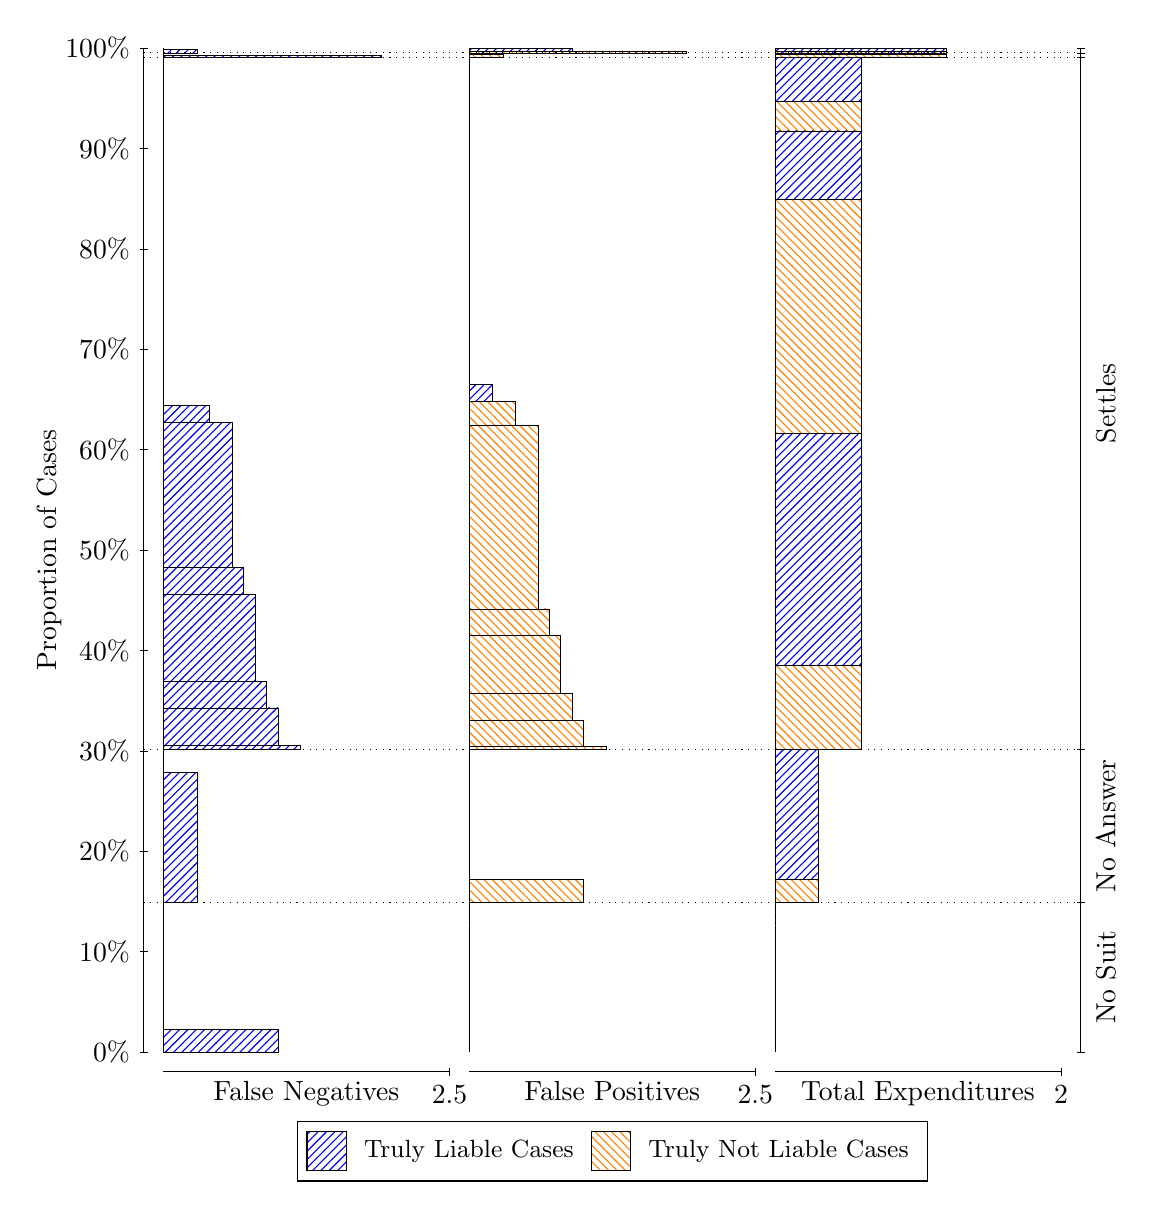
\begin{tikzpicture}
\draw[black, very thin] (1.5,1.75) -- (1.5,14.5);
\node[rotate=90, text=black, anchor=center] at (0.3, 8.125) {Proportion of Cases};
\draw[black, very thin] (1.45,1.75) -- (1.55,1.75);
\node[text=black, anchor=east] at (1.45, 1.75) {0\%};
\draw[black, very thin] (1.45,3.025) -- (1.55,3.025);
\node[text=black, anchor=east] at (1.45, 3.025) {10\%};
\draw[black, very thin] (1.45,4.3) -- (1.55,4.3);
\node[text=black, anchor=east] at (1.45, 4.3) {20\%};
\draw[black, very thin] (1.45,5.575) -- (1.55,5.575);
\node[text=black, anchor=east] at (1.45, 5.575) {30\%};
\draw[black, very thin] (1.45,6.85) -- (1.55,6.85);
\node[text=black, anchor=east] at (1.45, 6.85) {40\%};
\draw[black, very thin] (1.45,8.125) -- (1.55,8.125);
\node[text=black, anchor=east] at (1.45, 8.125) {50\%};
\draw[black, very thin] (1.45,9.4) -- (1.55,9.4);
\node[text=black, anchor=east] at (1.45, 9.4) {60\%};
\draw[black, very thin] (1.45,10.675) -- (1.55,10.675);
\node[text=black, anchor=east] at (1.45, 10.675) {70\%};
\draw[black, very thin] (1.45,11.95) -- (1.55,11.95);
\node[text=black, anchor=east] at (1.45, 11.95) {80\%};
\draw[black, very thin] (1.45,13.225) -- (1.55,13.225);
\node[text=black, anchor=east] at (1.45, 13.225) {90\%};
\draw[black, very thin] (1.45,14.5) -- (1.55,14.5);
\node[text=black, anchor=east] at (1.45, 14.5) {100\%};

\draw[black, very thin] (13.4,1.75) -- (13.4,14.5);
\draw[black, very thin] (13.35,1.75) -- (13.45,1.75);
\node[anchor=west] at (13.35, 1.75) {};
\draw[black, very thin] (13.35,3.6464) -- (13.45,3.6464);
\node[anchor=west] at (13.35, 3.6464) {};
\draw[black, very thin] (13.35,5.5927) -- (13.45,5.5927);
\node[anchor=west] at (13.35, 5.5927) {};
\draw[black, very thin] (13.35,14.384) -- (13.45,14.384);
\node[anchor=west] at (13.35, 14.384) {};
\draw[black, very thin] (13.35,14.439) -- (13.45,14.439);
\node[anchor=west] at (13.35, 14.439) {};
\draw[black, very thin] (13.35,14.5) -- (13.45,14.5);
\node[anchor=west] at (13.35, 14.5) {};

\draw[black, very thin, pattern color=blue, pattern=north east lines] (1.75,1.75) rectangle (3.2033,2.0387);
\draw[black, very thin, pattern color=orange, pattern=north west lines] (1.75,2.0387) rectangle (1.75,3.6464);
\draw[black, very thin, pattern color=blue, pattern=north east lines] (1.75,3.6464) rectangle (2.186,5.3002);
\draw[black, very thin, pattern color=orange, pattern=north west lines] (1.75,5.3002) rectangle (1.75,5.5927);
\draw[black, very thin, pattern color=blue, pattern=north east lines] (1.75,5.5927) rectangle (3.494,5.6393);
\draw[black, very thin, pattern color=blue, pattern=north east lines] (1.75,5.6393) rectangle (3.2033,6.1186);
\draw[black, very thin, pattern color=blue, pattern=north east lines] (1.75,6.1186) rectangle (3.058,6.4595);
\draw[black, very thin, pattern color=blue, pattern=north east lines] (1.75,6.4595) rectangle (2.9127,7.5611);
\draw[black, very thin, pattern color=blue, pattern=north east lines] (1.75,7.5611) rectangle (2.7673,7.8999);
\draw[black, very thin, pattern color=blue, pattern=north east lines] (1.75,7.8999) rectangle (2.622,9.7442);
\draw[black, very thin, pattern color=blue, pattern=north east lines] (1.75,9.7442) rectangle (2.3313,9.9641);
\draw[black, very thin, pattern color=orange, pattern=north west lines] (1.75,9.9641) rectangle (1.75,14.384);
\draw[black, very thin, pattern color=blue, pattern=north east lines] (1.75,14.384) rectangle (4.5113,14.403);
\draw[black, very thin, pattern color=orange, pattern=north west lines] (1.75,14.403) rectangle (1.75,14.439);
\draw[black, very thin, pattern color=blue, pattern=north east lines] (1.75,14.439) rectangle (2.186,14.481);
\draw[black, very thin, pattern color=orange, pattern=north west lines] (1.75,14.481) rectangle (1.75,14.5);
\draw[black, very thin, pattern color=orange, pattern=north west lines] (5.6333,1.75) rectangle (5.6333,3.3577);
\draw[black, very thin, pattern color=blue, pattern=north east lines] (5.6333,3.3577) rectangle (5.6333,3.6464);
\draw[black, very thin, pattern color=orange, pattern=north west lines] (5.6333,3.6464) rectangle (7.0867,3.939);
\draw[black, very thin, pattern color=blue, pattern=north east lines] (5.6333,3.939) rectangle (5.6333,5.5927);
\draw[black, very thin, pattern color=orange, pattern=north west lines] (5.6333,5.5927) rectangle (7.3773,5.6276);
\draw[black, very thin, pattern color=orange, pattern=north west lines] (5.6333,5.6276) rectangle (7.0867,5.9644);
\draw[black, very thin, pattern color=orange, pattern=north west lines] (5.6333,5.9644) rectangle (6.9413,6.3053);
\draw[black, very thin, pattern color=orange, pattern=north west lines] (5.6333,6.3053) rectangle (6.796,7.0369);
\draw[black, very thin, pattern color=orange, pattern=north west lines] (5.6333,7.0369) rectangle (6.6507,7.3758);
\draw[black, very thin, pattern color=orange, pattern=north west lines] (5.6333,7.3758) rectangle (6.5053,9.7075);
\draw[black, very thin, pattern color=orange, pattern=north west lines] (5.6333,9.7075) rectangle (6.2147,10.012);
\draw[black, very thin, pattern color=blue, pattern=north east lines] (5.6333,10.012) rectangle (5.924,10.232);
\draw[black, very thin, pattern color=blue, pattern=north east lines] (5.6333,10.232) rectangle (5.6333,14.384);
\draw[black, very thin, pattern color=orange, pattern=north west lines] (5.6333,14.384) rectangle (6.0693,14.42);
\draw[black, very thin, pattern color=blue, pattern=north east lines] (5.6333,14.42) rectangle (5.6333,14.439);
\draw[black, very thin, pattern color=orange, pattern=north west lines] (5.6333,14.439) rectangle (8.3947,14.458);
\draw[black, very thin, pattern color=blue, pattern=north east lines] (5.6333,14.458) rectangle (6.9413,14.5);
\draw[black, very thin, pattern color=orange, pattern=north west lines] (9.5167,1.75) rectangle (9.5167,3.3577);
\draw[black, very thin, pattern color=blue, pattern=north east lines] (9.5167,3.3577) rectangle (9.5167,3.6464);
\draw[black, very thin, pattern color=orange, pattern=north west lines] (9.5167,3.6464) rectangle (10.062,3.939);
\draw[black, very thin, pattern color=blue, pattern=north east lines] (9.5167,3.939) rectangle (10.062,5.5927);
\draw[black, very thin, pattern color=orange, pattern=north west lines] (9.5167,5.5927) rectangle (10.607,6.6611);
\draw[black, very thin, pattern color=blue, pattern=north east lines] (9.5167,6.6611) rectangle (10.607,9.607);
\draw[black, very thin, pattern color=orange, pattern=north west lines] (9.5167,9.607) rectangle (10.607,12.582);
\draw[black, very thin, pattern color=blue, pattern=north east lines] (9.5167,12.582) rectangle (10.607,13.449);
\draw[black, very thin, pattern color=orange, pattern=north west lines] (9.5167,13.449) rectangle (10.607,13.825);
\draw[black, very thin, pattern color=blue, pattern=north east lines] (9.5167,13.825) rectangle (10.607,14.384);
\draw[black, very thin, pattern color=orange, pattern=north west lines] (9.5167,14.384) rectangle (11.697,14.42);
\draw[black, very thin, pattern color=blue, pattern=north east lines] (9.5167,14.42) rectangle (11.697,14.439);
\draw[black, very thin, pattern color=orange, pattern=north west lines] (9.5167,14.439) rectangle (11.697,14.458);
\draw[black, very thin, pattern color=blue, pattern=north east lines] (9.5167,14.458) rectangle (11.697,14.5);
\draw[black, dotted] (1.5,3.6464) -- (13.4,3.6464);
\draw[black, dotted] (1.5,5.5927) -- (13.4,5.5927);
\draw[black, dotted] (1.5,14.384) -- (13.4,14.384);
\draw[black, dotted] (1.5,14.439) -- (13.4,14.439);
\draw[black, very thin] (1.75,1.5) -- (5.3833,1.5);
\node[text=black, anchor=north] at (3.5667, 1.5) {False Negatives};
\draw[black, very thin] (5.3833,1.45) -- (5.3833,1.55);
\node[text=black, anchor=north] at (5.3833, 1.45) {2.5};

\draw[black, very thin] (5.6333,1.5) -- (9.2667,1.5);
\node[text=black, anchor=north] at (7.45, 1.5) {False Positives};
\draw[black, very thin] (9.2667,1.45) -- (9.2667,1.55);
\node[text=black, anchor=north] at (9.2667, 1.45) {2.5};

\draw[black, very thin] (9.5167,1.5) -- (13.15,1.5);
\node[text=black, anchor=north] at (11.333, 1.5) {Total Expenditures};
\draw[black, very thin] (13.15,1.45) -- (13.15,1.55);
\node[text=black, anchor=north] at (13.15, 1.45) {2};

\node[text=black, centered, rotate=90] at (13.72, 2.6982) {No Suit};
\node[text=black, centered, rotate=90] at (13.72, 4.6196) {No Answer};
\node[text=black, centered, rotate=90] at (13.72, 9.9882) {Settles};



\draw (7.449999999999999,1.5) node[draw=none] (baseCoordinate) {};
\begin{scope}[align=center]
        \matrix[scale=0.5, draw=black, below=0.5cm of baseCoordinate, nodes={draw}, column sep=0.1cm]{
            \node[rectangle, draw, minimum width=0.5cm, minimum height=0.5cm, pattern color=blue, pattern=north east lines] {}; &
            \node[draw=none, font=\small, text=black] (B) {Truly Liable Cases}; &
            \node[rectangle, draw, minimum width=0.5cm, minimum height=0.5cm, pattern color=orange, pattern=north west lines] {}; &
            \node[draw=none, font=\small, text=black] (B) {Truly Not Liable Cases}; \\
            };
\end{scope}

\end{tikzpicture}
\end{document}